\chapter{Описание практической части}
\label{sec:Chapter4} \index{Chapter4}

	Алгоритм, описанный в предыдущей главе был реализован на языках Matlab и Python. В Matlab использовались  стандартные библиотеки, в Python - библиотеки numpy и scipy. 
	
\section{Калибровка алгоритма}

	Необходимым критерием для статистической оценке псевдоточечных целей является их наличие в диапозоне от 100 до 1000. Верхняя граница определяется возможностью вычислительных ресурсов ЭВМ. Для достижения поставленного критерия была выполнена калибровка алгоритма. Она заключается в установлении динамического порога при отборе псевдодочечных целей, который зависит от значения коэффициента эксцесса. Также был реализован динамический диапозон размеров клеток сетки, который зависит от размера входного изображения. Калибровка выполнялась на 22 радиолокационных снимков разного частотного диапазона.

\section{Верификация алгоритма}

	Для верификации работы алгоритма был выбран полигон с уголковыми отражателями Surat, который находится в Австралии. Полученные с уголковых отражателей значения разрешений сравнивались с результатом работы алгоритма. Соответствующие ошибки в определении разрешений представлены в таблице \ref{tab:errors}.
	
\begin{table}[]
    \centering
    \caption{Относительные ошибки в определении разрешений}
    \label{tab:errors}
    \begin{tabular}{|c|c|c|c|c|}
        \hline
        Название РСА  & Кол-во снимков  & Сигнал/шума, дБ  & $\epsilon$ & $\epsilon$  \\ \hline
        Iceye X-диапазон      & 7  & 43.9 & 1.09 & 1.80  \\ \hline
        Novasar-1 S-диапазон  & 11 & 38.7 & 0.73 & 3.11\\ \hline
        Sentinel-1 C-диапазон & 4  & 32   & 0.50 & 1.40  \\ \hline
        \multicolumn{3}{|c|}{Среднее значение} &  0.803 & 2.386 \\ \hline
    \end{tabular}
\end{table}

\section{Валидация алгоритма}

	В качестве валидации был обработан снимок Sentinel-1 в отсутсвии какой-либо информации о снимаемой сцене и, соответсвенно, в отсутвии уголковых отражателей. Результат обработки представлен на рисунке \ref{fig:senti}.
	
\begin{figure}[ht]
    \centering
    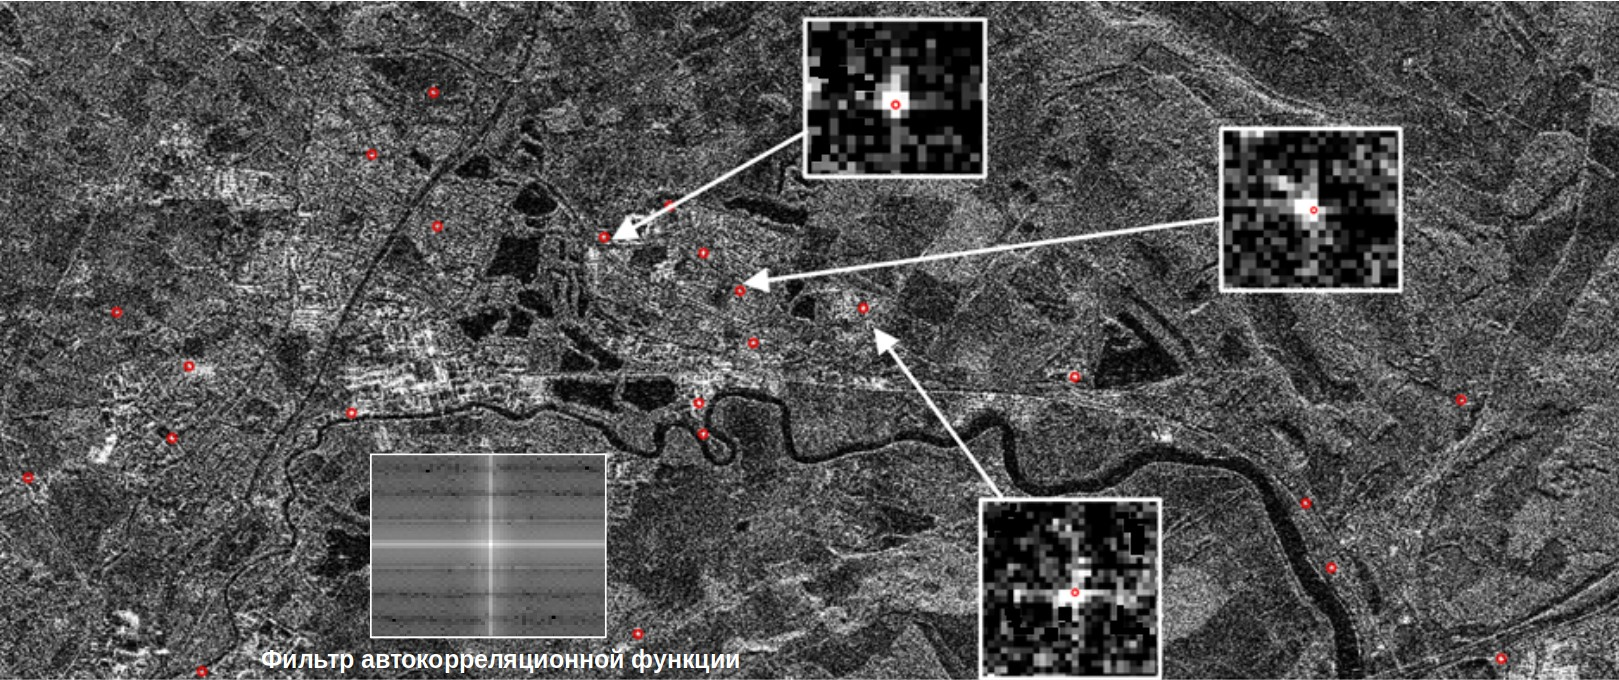
\includegraphics[width=1\textwidth]{senti.png}
    \caption{Снимок с РСА Sentinel}
    \label{fig:senti}
\end{figure}

	Полученные распределения и разрешения представлены на рисунке \ref{fig:distr}.	

\begin{figure}[ht]
    \centering
    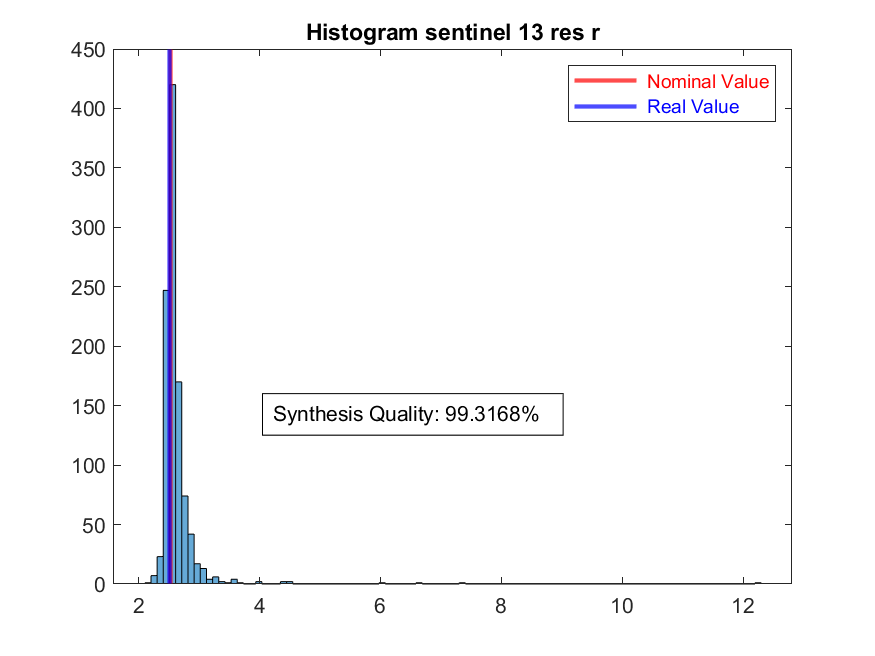
\includegraphics[width=1\textwidth]{distr.png}
    \caption{Гистограмма распределения разрешений}
    \label{fig:distr}
\end{figure}

	Полученные разрешения по дальности и по азимуту оказались равными 2.422 м 3.524 м соотвественно. При этом предельная разрешающая способность РСА равна 2.525 м и 3.56 м, что говорит о хорошем качестве синтеза изображения. То есть, коэффициент ухудшения равен соотвественно ... и ... .	

\newpage
